\documentclass{article}
\usepackage[utf8]{inputenc}
\usepackage[brazilian]{babel}
\usepackage{geometry}
\geometry{a4paper, total={150mm,240mm}, top=25mm}
\usepackage{graphicx}
\usepackage{titling}
\usepackage{float}
\usepackage{natbib}
\usepackage{setspace}
\usepackage{algorithm}
\usepackage{algpseudocode}
\usepackage{amsfonts}
\onehalfspacing

\title{Trabalho 2 - Diagrama de Voronoi}
\author{Kleyton da Costa (2312730)}
\date{\today}
 
\usepackage{fancyhdr}
\fancypagestyle{plain}{%  the preset of fancyhdr 
    \fancyhf{} % clear all header and footer fields
    \fancyfoot[R]{
\includegraphics[width=3cm]{di.png}}
    \fancyfoot[L]{\today}
    \fancyhead[L]{Geometria Computacional}
    \fancyhead[R]{\theauthor}
}
\makeatletter
\def\@maketitle{%
  \newpage
  \null
  \vskip 1em%
  \begin{center}%
  \let \footnote \thanks
    {\LARGE \@title \par}%
    \vskip 1em%
    %{\large \@date}%
  \end{center}%
  \par
  \vskip 1em}
\makeatother

\begin{document}

\maketitle

\noindent\begin{tabular}{@{}ll}
    Aluno & \theauthor \\
    Professor &  Waldemar Celes (DI/PUC-Rio)
\end{tabular}

\section{Motivação}

Este trabalho tem como objetivo implementar um diagrama de Voronoi a partir de um conjunto de pontos que não possui degenerações. Para este trabalho foi utilizado o algoritmo incremental.

\section{Metodologia}

A região de Voronoi de um determinando ponto $p$, que faz parte de uma nuvem de pontos $S$, é o conjunto de todos os pontos $x$ que estão mais próximos de $p$ do que de qualquer outra região $q$ que também pertence a $S$. Sendo esta distância computada pela norma entre $x$ e $p$ e entre $x$ e $q$, podemos definir a região de Voronoi de $p$ como sendo 

\begin{equation}
  Vor(p) = \{x\in \mathbb{R}^{2} ~|~ \|x-p\| \leq \|x-q\|, ~~\forall~q\in S \}
\end{equation}

Dessa maneira, quando o nosso objetivo é particionar o plano em diferentes regiões com base na distância entre os pontos, podemos construir o Diagrama de Voronoi, ou seja, os limites que são definidos quando computamos as regiões de Voronoi para todos os $p_{i}$ pontos de uma nuvem de pontos $S$.

O algoritmo incremental para a construção do diagrama de Voronoi, proposto por Peter Green e Robin Sibson em 1977, foi considerado para os experimentos realizados neste trabalho. Assim como o método incremental utilizado para a construção do fecho convexo e das triangulações, a ideia é considerar um diagrama de Voronoi construído para um determinado número $i$ de posições e adicionar um novo local $p$ ao plano, convertando em seguida o diagrama de Voronoi construído para incluir a região de Voronoi $p$. Com uma complexidade assintótica $O(n^{2})$, o funcionamento do algoritmo é descrito como

\begin{quotation}
  \noindent \textit{Dado $Vor(S)$, encontrar $Vor(p_{i})$ que contenha um novo ponto $p$. Desenhar um segmento $x_{1}x_{2}$ para a bissetora $\overline{p_{1}p}$. Continuando a partir de $x_{2}$, construir a região de Voronoi de $p$ segmento por segmento até que acontece o retorno a $x_{1}$. Por fim, deve-se remover o subdiagrama que está localizado dentro da região poligonal para se obter o novo diagrama de Voronoi, mas que passa a conter o ponto $p$. Esse processo pode ser observado na Figura \ref{fig:incremental}} 
\end{quotation}

\begin{figure}[H]
  \centering
  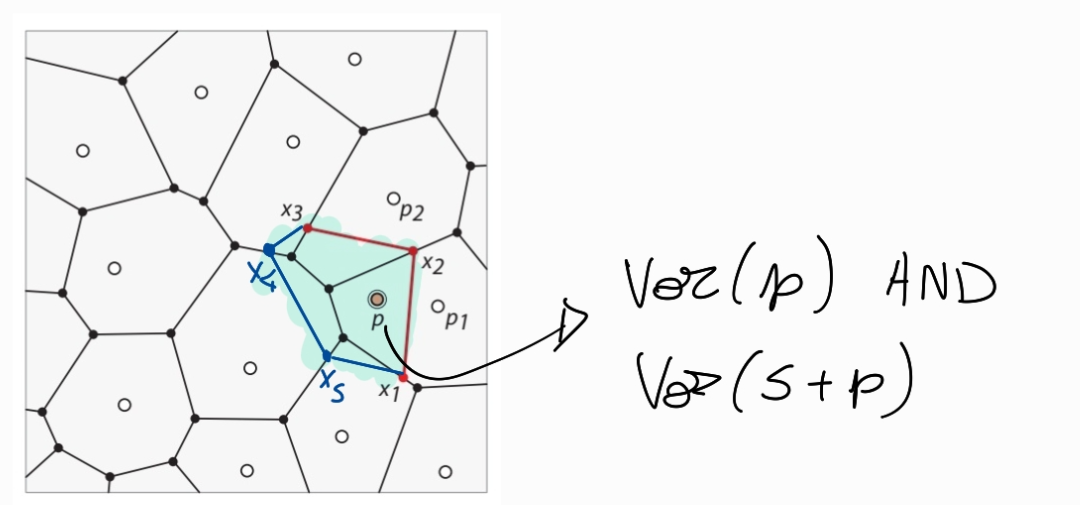
\includegraphics[scale=0.3]{incremental.png}
  \caption{Desenho do funcionamento do algoritmo incremental}
  \label{fig:incremental}
\end{figure}


\section{Experimentos}

Utilizando as nuvens de pontos disponibilizadas, chegamos até a configuração de resultados apresentada nas Figuras \ref{fig:nuvem1} e \ref{fig:nuvem2}.

\begin{figure}[H]
  \centering
  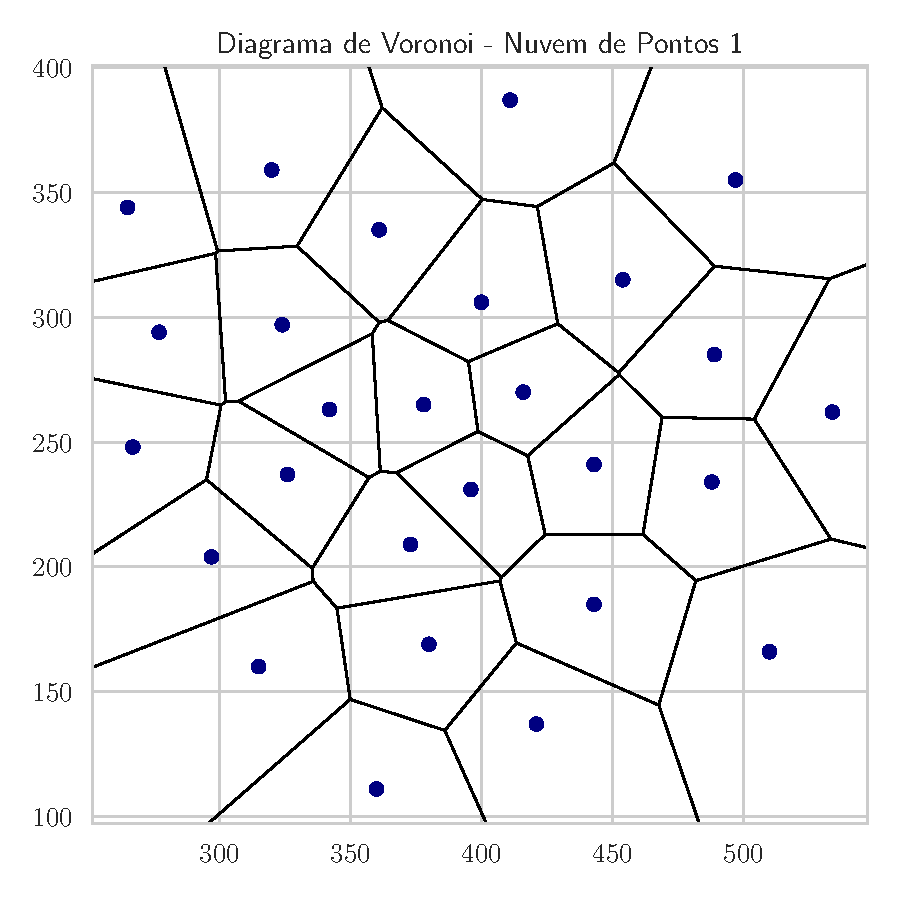
\includegraphics[scale=0.6]{plot_voronoi1.pdf}
  \caption{Diagrama de Voronoi para a nuvem de pontos 1}
  \label{fig:nuvem1}
\end{figure}

\begin{figure}[H]
  \centering
  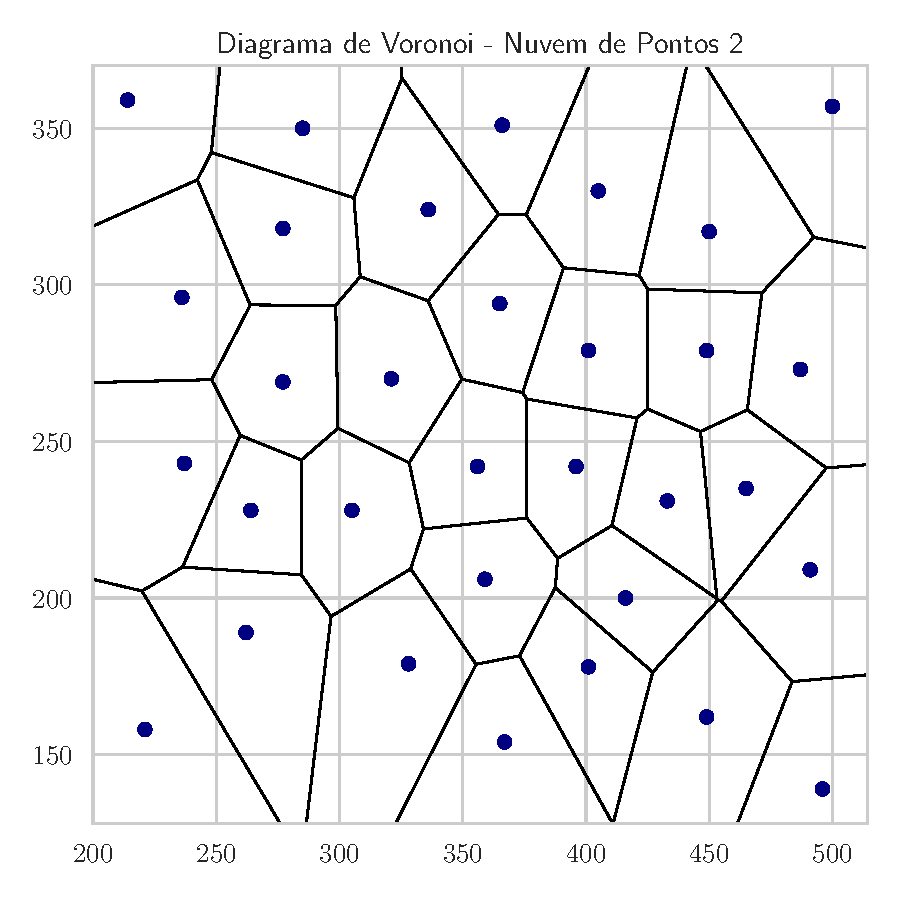
\includegraphics[scale=0.6]{plot_voronoi2.pdf}
  \caption{Diagrama de Voronoi para a nuvem de pontos 2}
  \label{fig:nuvem2}
\end{figure}


\section{Considerações Finais}

Neste trabalho foi apresentada a implemetação do algoritmo de Voronoi considerando o algoritmo incremental. A complexidade assintótica do algoritmo sendo $O(n^2)$ traz certas limitações em termos de tempo de processamento para conjuntos de dados maiores. No entanto, o algoritmo consegue gerar os resultados de maneira satisfatória.

\bibliographystyle{apa}
\bibliography{work2-voronoi/references.bib}

\end{document}